На рисунке \ref{fig:server} представлен внешний вид пользовательского веб-интерфейса.\par
\begin{figure}[ht]
    \centering
    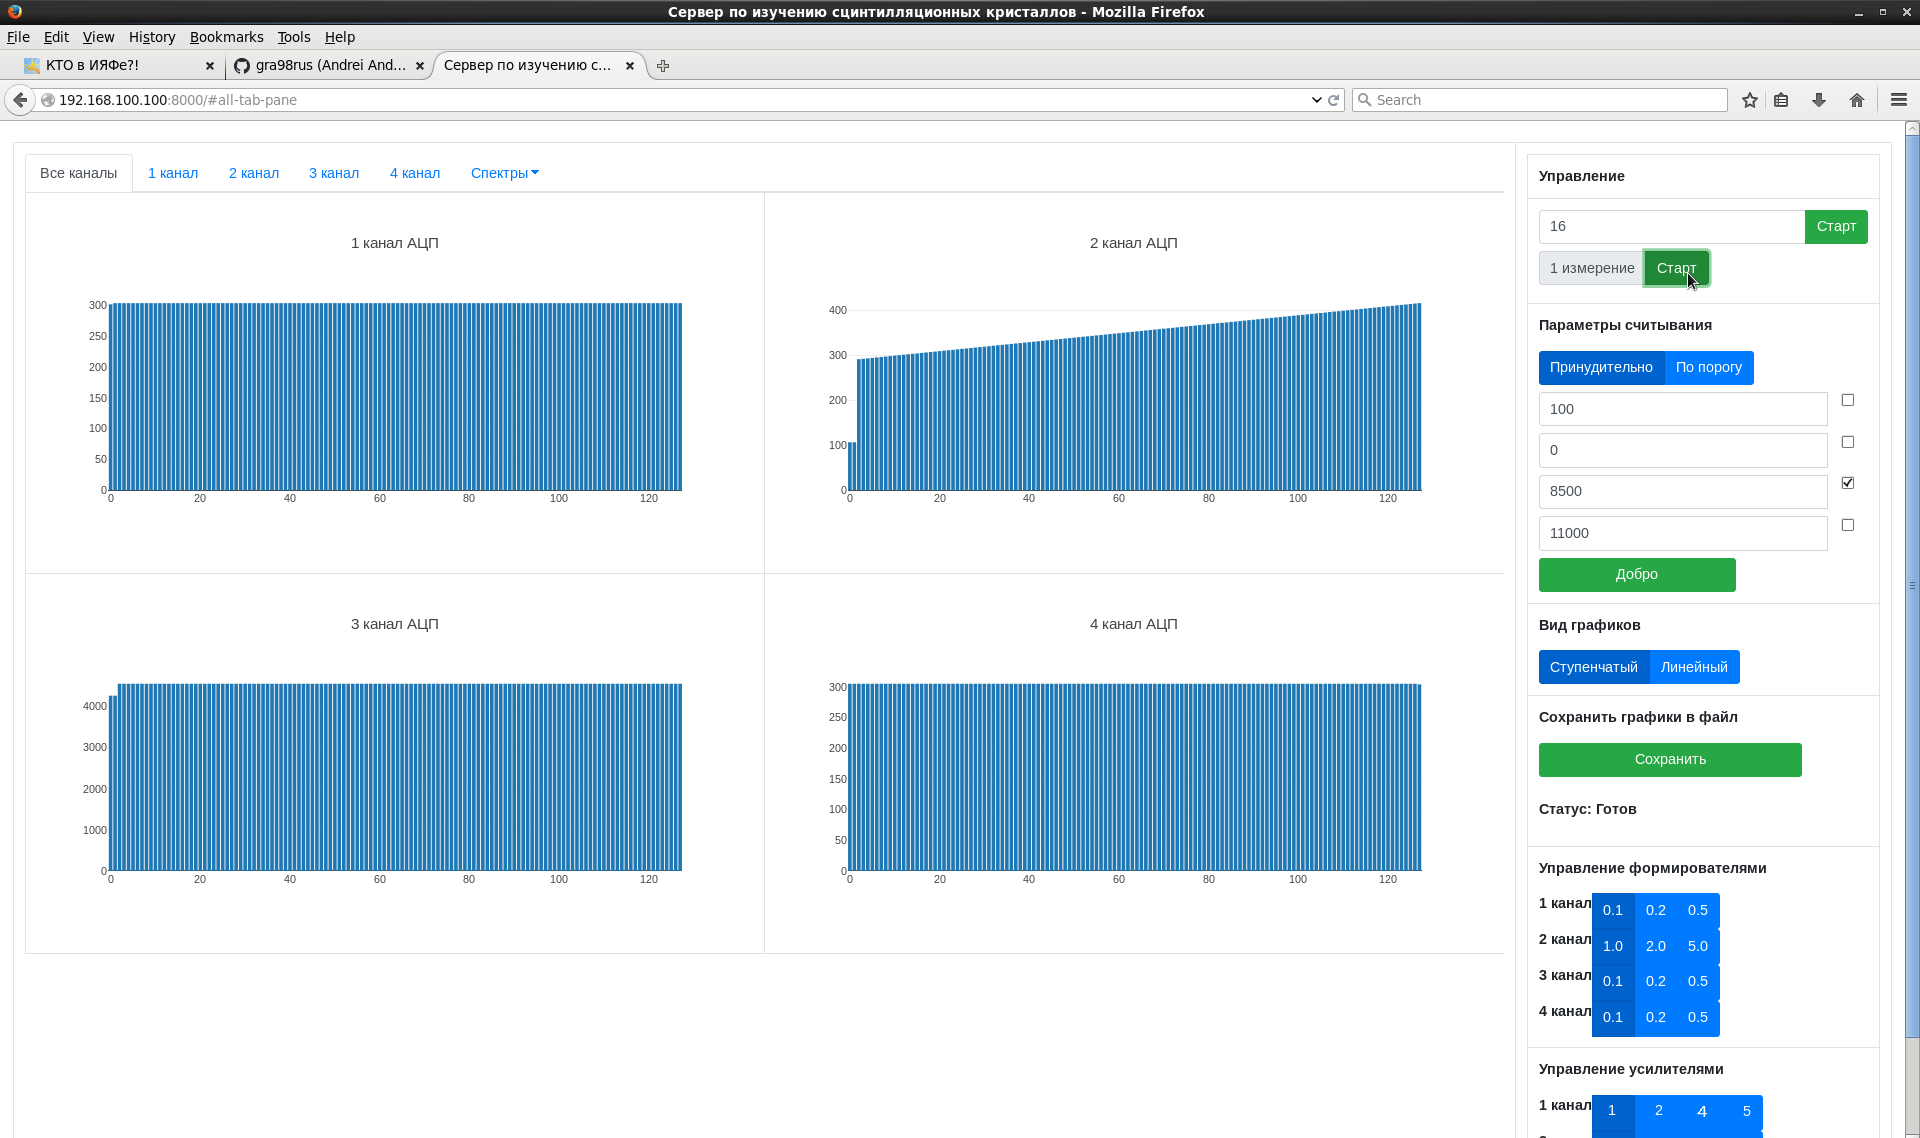
\includegraphics[width=1\linewidth]{server.jpg}
    \caption{Пользовательский веб-интерфейс}
    \label{fig:server}
\end{figure}
На главной странице расположены область с графиками и панель управления стендом. В верхней части страницы предусмотрены вкладки для переключения между графиками. Также здесь расположена вкладка ``Спектры'', где оператор может управлять гистограммами: добавить новую с выбранными параметрами или удалить существующие. Среди параметров присутствуют следующие параметры: выбранный канал АЦП, количество корзин (от 32 до 4096) и тип гистограммы (по максимальному значению амплитуды или же по амплитуде опорной точки, которую также можно задать).\par
На боковой панели управления оператор может задавать следующие параметры:\par
\begin{itemize}
    \item количество запусков;
    \item тип считывания (принудительный или по порогу);
    \item значения порогов для каждого канала АЦП, а также по каким каналам возможно срабатывание;
    \item вид графиков (ступенчатый или линейный);
    \item коэффициент усиления сигналов и времена формирования каждого входного сигнала.
\end{itemize}\par
Также реализована возможность сохранять данные в файл для последующего анализа.\par
Разработка велась с использованием языков JavaScript, HTML и CSS. \par
